\documentclass[UTF8,10pt]{ctexart}

\usepackage{multicol}
\usepackage{geometry}
\usepackage{fancyhdr}
\usepackage{graphicx}
\usepackage{authblk}
\usepackage{enumerate}
\usepackage{booktabs}
\usepackage{amsmath}
\usepackage{pythonhighlight}

\setlength\columnsep{0.6cm}
\geometry{left=1.2cm,right=1.2cm,top=2.5cm,bottom=1.8cm}
\title{\vspace{-2cm}HPC101\ 实验3\quad 实验报告}
\author[ ]{张云轩*\quad 3200105087}
%\affil[ ]{3200105087}
\affil[*]{信息与电子工程学院\quad 信息工程}
\affil[*]{竺可桢学院\quad 工程教育高级班}

\date{\today}

\pagestyle{fancy}
%清除原页眉页脚样式
\fancyhf{} 
%R:页面右边;O:奇数页;\leftmark:表示“一级标题”
\fancyhead[RO]{\leftmark}
%L:页面左边;E:偶数页;\rightmark:表示“二级标题”
\fancyhead[LE]{\rightmark}
%C:页面中间
\fancyhead[CO, CE]{HPC101\ 实验3\quad 实验报告}
%同上,但是不同位置放置不同信息
\fancyhead[LO, RE]{}
% 设置页脚,页眉的位置上也可以放置页码
\fancyfoot[RO, LE]{\thepage}
\fancyfoot[LO, RE]{}
% 设置页眉页脚横线及样式
%页眉线宽,设为0可以去页眉线
\renewcommand{\headrulewidth}{0.1mm} 
%页脚线宽,设为0可以去页眉线
\renewcommand{\footrulewidth}{0mm} 

\begin{document}

\maketitle

\section{实验任务与要求}
\begin{enumerate}[1]
    \item 使用GPU和CUDA Runtime API加速卷积运算
    \item 测试计算正确性和加速比
    \item 提交代码和简要的思路
\end{enumerate}

\section{实验环境}
\begin{center}
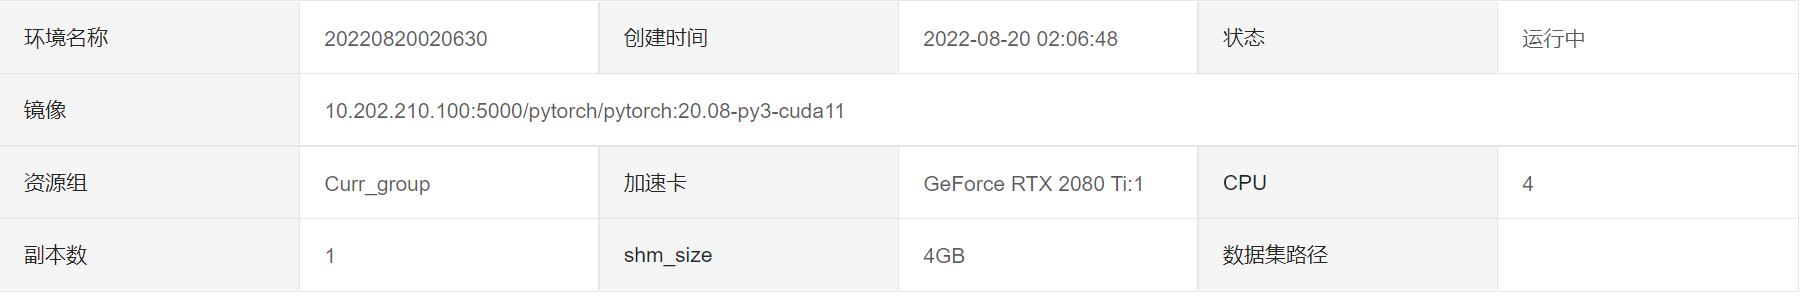
\includegraphics[scale=0.58]{img/1.PNG}
\end{center}
\paragraph{CPU} Intel(R) Xeon(R) Gold 6226R CPU @ 2.90GHz x4
\paragraph{Memory} 251GB
\paragraph{GPU} Nvidia(R) GeForce RTX 2080Ti with CUDA 11.0

\section{问题重述}
对于输入的两个四维张量$a[N][H][W][CI]$和$w[KH][KW][CI][CO]$,其中$N$表示输入张量的批大小batch\_size;$H$、$W$分别表示输入张量的高和宽;$CI$表示输入张量的通道数;$KH$、$KW$分别表示卷积核的高和宽;$CO$表示输出张量的通道数。输入张量$a$与卷积核$w$的卷积运算定义如下:
\begin{equation}
    (a*w)(n, h, w, co)=\sum_{i=-(KH)/2}^{(KH)/2} \sum_{j=-(KW)/2}^{(KW)/2} \sum_{ci=0}^{CI} a[n][h+i][y+j][ci]·w[i][j][ci][co]
\end{equation}
计算$a$与$w$的卷积运算结果$b[N][H][W][CO]$,它也是一个四维向量。

\section{实验步骤}
\subsection{Baseline基准测试}
\begin{python}
编译命令:nvcc -o conv conv.cu -O3 -cudart=shared -Xcompiler -fopenmp --ptxas-options=-v
\end{python}
\begin{python}
Correct
CUDA time: 11507.5 ms
accelerate ratio: 1.9118
\end{python}
baseline的运行时间为11.5秒,相比CPU版本加速了约一倍。

\subsection{im2col算法:将卷积运算转化为通用矩阵乘法(GEMM)}
张量卷积可以看成移动窗口操作。卷积核是窗口,每次在输入图像上移动一定的距离,在每个位置上与窗内每个对应位置元素点乘,然后将各个元素的点乘结果累加起来,作为这个窗口内的结果。这个首先对应位置元素相乘,然后相乘结果累加的操作与矩阵乘法的计算过程十分类似。因此,可以考虑以一定的方式将张量展开为矩阵,然后以矩阵乘法代替卷积操作,最后再以一定的方式将结果矩阵变换为结果张量。对通用矩阵乘法(GEMM)的并行优化有一套成熟的理论,因此可以通过这种转换加速卷积的计算。事实上,CUDA的神经网络算子库cuDNN内对张量卷积的实现就是使用的这种方法。

首先考虑二维张量的卷积过程。将将每一次滑动窗口框选的子矩阵展开为一维向量,然后纵向排列,得到一个行数量为滑动窗口数$a$、列数量为每个滑动窗口内元素数$b$(卷积核元素数)的矩阵$A_{ab}$。然后将卷积核直接展开为列向量$W_{b1}$。A与W相乘,得到一个$a$行1列的列向量$B_{a1}$,将这个列向量按先行后列、从左向右、从上到下的顺序重排成一个矩阵,这就是输入矩阵与卷积核的卷积结果。

对于多通道的输入张量和卷积核,即三维张量输入与三维张量卷积核卷积,只需要将每个滑动窗口内每个通道展开的行向量头尾接在一起拼成一个更长的行向量,然后每个滑动窗口的行向量纵向排列得到矩阵;卷积核的每个通道展开成的列向量首尾连接在一起拼成一个更长的列向量,每一条(一个滑动窗口)相乘的过程其实就是对应通道的输入张量元素和卷积核点乘后累加。最终得到的结果矩阵与单通道卷积没有区别。

对于多输出通道(多个卷积核)卷积,即三维张量输入与四维张量卷积核卷积,只需要按上一步处理输入张量和每个输出通道的卷积核,然后把每个通道的卷积核展开成的列向量横向排布在一起,得到一个卷积核矩阵$W_{bc}$,其中$b$代表每个滑动窗口内元素数,$c$代表输出通道数。这样矩阵乘法可以得到一个结果矩阵$B_{ac}$。将其分解为一条一条的列向量,每个列向量都依据上述单通道 的方法转化为单输出通道的卷积结果,即每个列向量都是一个输出通道的结果,在z方向上排布在一起,就是多输出通道卷积的卷积结果。

最后,对于多批输入,将每一批输入展开为的矩阵在纵向拼接在一起,然后将结果矩阵在纵向拆开为单批的结果矩阵,其余处理都没有区别。

在进行这项操作的时候,将目标内存开设在显存上,然后利用GPU开多个线程加速矩阵构造过程。具体实现过程见核函数cuda\_im2col\_a\_kernel、cuda\_im2col\_w\_kernel、cuda\_col2im\_b\_kernel及注释。

对构造过程进行测试:
\begin{python}
编译命令:nvcc -o conv conv_im2col.cu -O3 -cudart=shared -Xcompiler -fopenmp --ptxas-options=-v
\end{python}
\begin{python}
CUDA time: 60.2167 ms  // 构造过程耗时60.2ms
\end{python}

\subsection{CUDA加速的通用矩阵乘法}
上一步已经把问题转化为了通用矩阵乘法,这一步利用CUDA并行加速矩阵乘法计算。
\subsubsection{矩阵切分与线程分配方法}
如下图所示,在本计算实例中,结果矩阵是$128000\times 128$的矩阵。我们将结果矩阵切分成$128\times 128$的小块,每个block计算其中一块。与block的划分类似,block内部的每个线程计算结果子矩阵中$16\times 16$的子子矩阵,这样每个block内有128个线程。
\begin{python}
dim3 grid_GEMM(b_mat_height/block_size_m, b_mat_width/block_size_n);    // block
dim3 block_GEMM(block_size_m/thread_size_y, block_size_n/thread_size_x);    // thread
cuda_GEMM_kernel<<<grid_GEMM, block_GEMM>>>(a_mat, w_mat, b_mat);
cudaDeviceSynchronize();
\end{python}
\begin{center}
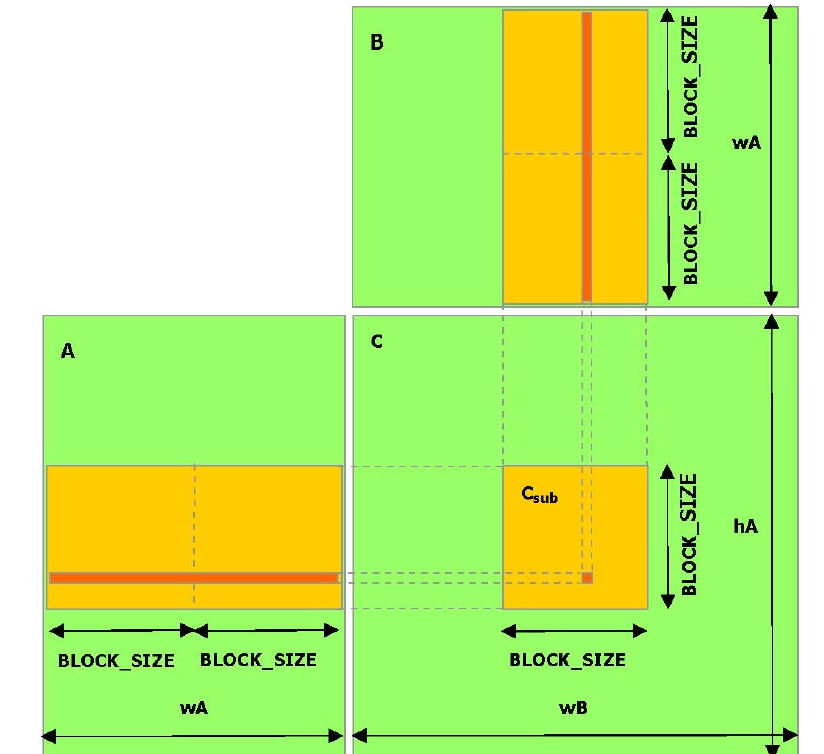
\includegraphics[scale=0.4]{img/2.png}
\end{center}

\subsubsection{利用shared memory和寄存器加速访存速度}
shared memory速度比global memory快得多,可以在整个block内共享,但是容量较小,无法一次存下所有计算所需数据。如下图所示,分多轮分批读取数据到shared memory。每轮结果对应累加即可得到最终结果。
\begin{center}
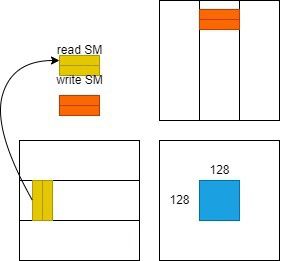
\includegraphics[scale=0.7]{img/3.jpg}
\end{center}

读取shared memory需要各个线程合作,分工读取不同部分,读取完后做一下线程同步,确保各个线程都读完了数据,之后的计算使用的数据是完整、正确的。

\begin{python}
// 读A
reinterpret_cast<float *>(&load_reg_a[0])[0]
=reinterpret_cast<float *>(&a_mat[k*(block_size_m*block_m_id+A_row_id_this_thread)+A_col_id_this_thread])[0];
As[0][A_col_id_this_thread][A_row_id_this_thread]=load_reg_a[0];
As[0][A_col_id_this_thread+1][A_row_id_this_thread]=load_reg_a[1];
As[0][A_col_id_this_thread+2][A_row_id_this_thread]=load_reg_a[2];
As[0][A_col_id_this_thread+3][A_row_id_this_thread]=load_reg_a[3];
// 读W
reinterpret_cast<float *>(&Ws[0][W_row_id_this_thread][W_col_id_this_thread])[0]
=reinterpret_cast<float *>(&w_mat[W_row_id_this_thread*n+W_col_id_this_thread])[0];
__syncthreads();    // 线程同步
\end{python}

与shared memory相比,寄存器的速度更快,但是容量更小,且只能每个线程独享。我们依然可以延续上述思路,如下图所示,每个线程分批多次读取shared memory中自己需要的数据到寄存器,之后将每批的计算结果累加,得到最终结果。由于每个数据都需要多次访问,因此一次访问shared memory、多次访问寄存器的时间成本是低于多次访问shared memory的。
\begin{center}
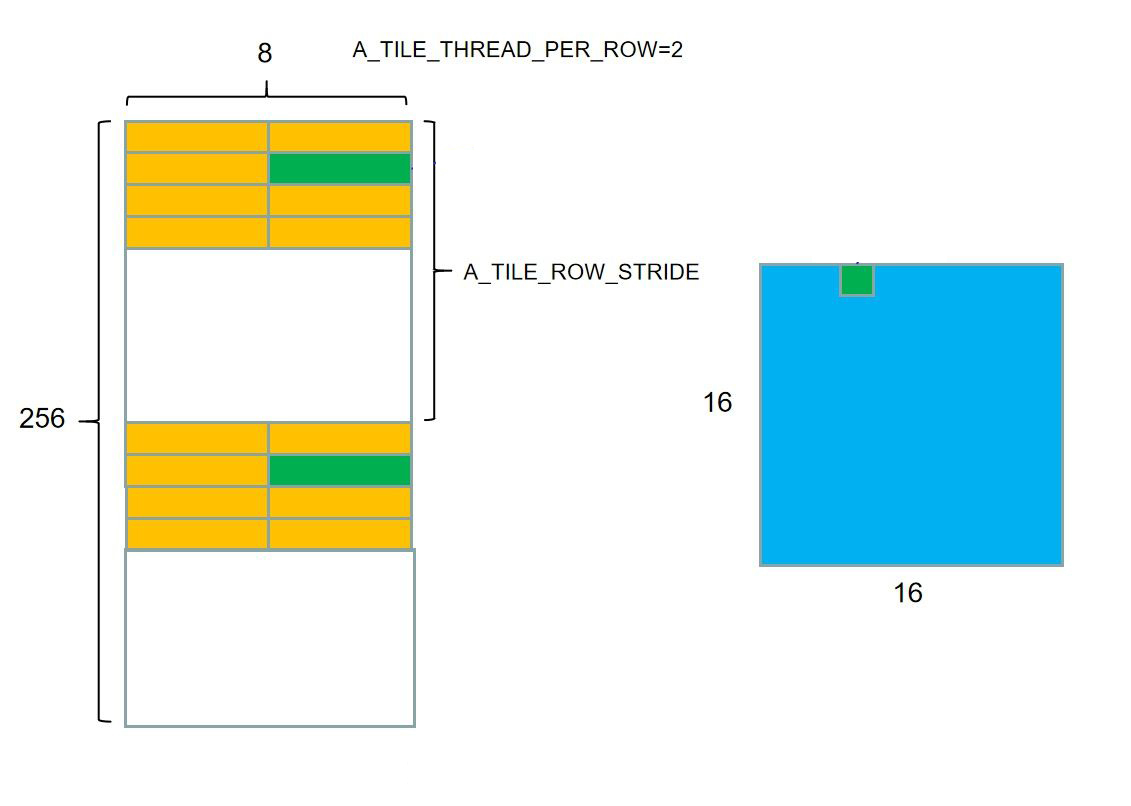
\includegraphics[scale=0.3]{img/4.jpg}
\end{center}

\begin{python}
#pragma unroll
for(int i=0; i<thread_size_y; i+=4)
  reinterpret_cast<float*>(&A_reg[0][i])[0]=reinterpret_cast<float*>(&As[0][0][thread_size_y*thread_y_id+i])[0];
#pragma unroll
for(int i=0; i<thread_size_x; i+=4)
  reinterpret_cast<float*>(&W_reg[0][i])[0]=reinterpret_cast<float*>(&Ws[0][0][thread_size_x*thread_x_id+i])[0];
\end{python}

\subsubsection{引入轮作方法隐藏访存延时}
将下一轮计算要使用的数据拷贝进shared memory的时候,这一轮的数据已经在shared memory里了。因此可以在下一次要用的数据拷贝的同时进行这一轮的计算,起到隐藏访存延时的作用。为此,需要在shared memory中开两倍的空间,分别用来存储该次和下一次的数据。

同理,每个线程的下一轮寄存器拷贝的同时也可以进行这一轮的计算,进一步隐藏访存延时。

\subsubsection{使用向量化数据类型在一个时钟周期内读取多个数据}
可以使用CUDA支持的float4向量数据类型读取方法在一个时钟周期内读取16个uint8\_t数据。为此需要使用reinterpret\_cast<float *>(\&Array[0])[0]将uint8\_t的指针强制类型转换为float4型。
\begin{python}
reinterpret_cast<float *>(&load_reg_a[0])[0]
=reinterpret_cast<float *>(&a_mat[k*(block_size_m*block_m_id+A_row_id_this_thread)+A_col_id_this_thread])[0];
\end{python}

\subsection{加速性能测试}
\subsubsection{AiStation}
\begin{python}
编译命令:nvcc -o conv conv_im2col_optimized.cu -O3 -cudart=shared -Xcompiler -fopenmp --ptxas-options=-v
\end{python}
\begin{python}
Correct
CUDA time: 199.512 ms
accelerate ratio: 416.015
\end{python}
前述的im2col构造算法耗时约60ms,因此计算时间约为140ms。

\subsubsection{slurm集群}
\begin{python}
编译命令:nvcc -o conv conv_im2col_optimized.cu -O3 -cudart=shared -Xcompiler -fopenmp --ptxas-options=-v
\end{python}
\begin{python}
Correct
CUDA time: 97.1198 ms
accelerate ratio: 411.862
\end{python}

\section{总结}
本实验利用CUDA加速了卷积运算,首先采用了im2col算法将卷积运算转化为通用矩阵乘法(GEMM),随后使用shared memory、寄存器加速、向量化读取以及多轮轮作隐藏访存延时等技术加速了GEMM计算,最终获得了416倍左右的加速比。


\end{document}